
\documentclass[a4paper,12pt]{article} % Changer la taille de police c'est ici

\usepackage{framed} % Marges
\usepackage[utf8]{inputenc} %francais
\usepackage[T1]{fontenc} %francais
\usepackage[french]{babel}  %francais
\usepackage{lmodern} % Pour changer le pack de police
\usepackage{makeidx} % Index
\usepackage{graphicx} % Figures
\usepackage{wrapfig} % Figures
\usepackage{amsmath} % Maths
\usepackage{amssymb} % symboles ?
\usepackage{bclogo} % ?????
\usepackage{hyperref}
\usepackage{stmaryrd}
\usepackage[top=2cm, bottom=2cm, left=2cm, right=2cm]{geometry} %Marges

\title{Rapport Interpolaspline}
\author{Interpolaspline}
\date{Avril 2020}

 \begin{document}
 \maketitle

\section{Linear Differential Equation}

\subsection{Splines de lissage uniformes}

Dans celle-ci. on traite des splines de lissage uniforme.
On considère une séquence de noeuds,  de coordonées en abscisse où pour n noeuds, nous avons $x_1 < x_2 < ... < x_n$. Ce qui diffère les splines de lissage unforme des autres splines, ce sont ses noeuds distribués de manière équidistante dans un intervalle déterminé, tel que $x_i+1 - x_i = h > 0, i = 1,...,n-1$ (comme l'illustre la figure ci-dessous, avec différentes splines de lissage).

\begin{figure}[htp]
    \centering
    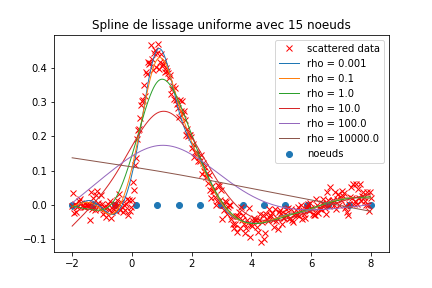
\includegraphics[width=10cm]{IMG_Tache1}
    \caption{Exemple de plusieurs courbes de lissages uniformes avec différents  $\rho$  }
    \label{fig:uniforme}
\end{figure}

Dans le fichier python dédié aux splines de lissage uniformes, un grand nombre de matrices sont calculées. Elles servent la création des splines de lissage. Plus d'information sur ces matrices se trouvent sur le polycopié de cours fourni par M. Biard aux étudiants L3 MI et disponible depuis sa page internet personelle (lien fourni en bibliographie).


Dans ces courbes de lissage uniformes, il existe un paramètre de lissage $\rho$ (soit rho sur la figure ci-dessus). Un de nos objectifs porte sur le calcul automatique optimal de ce paramètre par l'intermédiaire de notre application python.



\section{Bibliographie}
Luc Biard, Cours sur les splines de lissages
\href{http://www-ljk.imag.fr/membres/Luc.Biard/L3MI_cours/Splines.pdf}{Splines.pdf}
     \end{document}














